%\documentclass[twocolumn]{article}
\documentclass[conference]{IEEEtran}

\usepackage[left=2cm,top=1cm,right=2cm]{geometry}
\usepackage[pdftex]{graphicx}
\usepackage[utf8]{inputenc}
\usepackage{algorithmic}
\usepackage{algorithm}
%\usepackage{titlesec}
\usepackage{verbatim}

\begin{document}

\title{A Comparison of GPU and CPU Performance for Real-Time Fluid Simulation}

\author{\IEEEauthorblockN{Richard Monette}
\IEEEauthorblockA{Department of Systems and Computer Engineering \\
Carleton University, Ottawa, Ontario\\
Email: rmonette@connect.carleton.ca}
}

\maketitle

\begin{abstract}

In this paper we present our comparison of the performance of graphics processing unit (GPU) and central processing unit (CPU) hardware based implementations of a common fluid simulation algorithm. We implement the algorithm on both hardware architectures using the appropriate application programming interfaces in order to provide a fair comparison between optimized solutions in both scenarios. Performance metrics were gathered using current generation GPU and CPU hardware. We analyzed the design of both architectures highlighting which design features most affect performance in common throughput computing tasks. We put our results in context by comparing them to those results produced by other researchers. Finally, we present our suggestions for future optimization of both architectures at the hardware and software level.

\end{abstract}

\IEEEpeerreviewmaketitle

\section{Introduction}

As GPU hardware continues to gain ever more computational power, an increasing research effort is being invested in using the otherwise specialized hardware for general purpose computation tasks. The GPU uses a fundamentally different hardware architecture than the CPU, achieving its computational capacity through massive parallel processing instead of fast single thread performance. For tasks which exhibit data and thread level parallelism, it is possible to achieve superior performance through the use of a wide processing platform consisting of many relatively simple processors. In this paper, we independently examine the findings presented in the paper "Debunking the 100X GPU vs. CPU Myth", published by Lee et al.\cite{Lee:2010:DGV:1816038.1816021} To this end, we used the Nvidia Compute Unified Device Architecture (CUDA) SDK to implement a GPU version of the well known fluid simulation technique presented in the paper "Real-Time Fluid Dynamics for Games",  by Jos Stam.\cite{Stam:2003} We compare our novel GPU implementation with our CPU based, OpenMP multi-thread enhanced implementation of the same algorithm. We then compare our results to those presented by the prior authors. Finally, we examine the features in both the GPU and CPU architectures that account for our performance observations and provide suggestions for future improvement of those architectures. 

\section{Throughput Computing Applications}

Parallel processing approaches are best suited to those applications which exhibit data and thread level parallelism. In our particular case of fluid simulation it is possible to use thread level parallelism to perform the otherwise sequential processing of each fluid simulation cell. Additionally, SIMD computation units can be used to concurrently perform the calculations required for each cell. 

In their research, Lee et al. examined a range of throughput computing tasks including Single Precision General Matrix Multiplication (SGEMM), Monte Carlo integration (MC), convolution (Conv), Fast Fourier Transform (FFT), Scalar Alpha X Plus Y (SAXPY), Lattice Boltzmann method (LBM), constraint solving (Solv), sparse matrix vector multiplication (SPMM), GJK collision detection (GJK), radix sorting (Sort), ray casting (RC), in-memory tree structured index searching (Search), histogram computation (HIST) and bilateral filtering (Bilat). We leave it as an exercise to the reader to familiarize themselves with these techniques and will instead focus on presenting the fluid simulation technique used in this paper.\cite{Asanovic:2006}\cite{Bienia:2008}\cite{Chen:2008}\cite{IMPACT}

\subsection{Real-Time Simulation of Fluid Dynamics}

The standard method for calculating the behavior of fluids is to use the Navier-Stokes equations. These equations, which have existed since the 1800's, allow for precise calculation of the behavior of most fluids found in nature. Because they can only be analytically solved for the most simple cases, there was little progress made in using them until the advent of efficient digital computation machinery. 

\begin{figure}[b]
\begin{equation}
\frac{\delta u}{\delta t} = -(u \cdot \bigtriangledown)u + v \bigtriangledown^2u + f
\end{equation}

\begin{equation}
\frac{\delta \rho}{\delta t} = -(u \cdot \bigtriangledown)\rho + \kappa \bigtriangledown^2\rho + S
\end{equation}
\caption{The Navier-Stokes equations for velocity in a compact vector notation (top) and the equation for a density moving through the velocity field (bottom).\cite{Stam:2003}}
\end{figure}

At each time step in the simulation we model the fluid as a field of velocity vectors which describe the flow of the fluid. In order to visualize this movement, a density of material is introduced into the system. This density moves through the fluid according to the velocity vectors. Density can be visualized as a gradient between black and white or the colors that are most appropriate for the fluid type (smoke, fire, water) being simulated. 

\subsubsection{GPU Implementation Details}

In implementing our GPU version of the fluid simulation algorithm, we found that the main constraint on performance was memory bandwidth. In order to achieve better performance we made use of the special purpose texture sampling hardware available on the GTX280. The texture fetch functionality has additional caches and is optimized for fetching in the regular patterns which characterize the update cycles of our fluid simulation algorithm.\cite{Sanders:2001} In order to allow the same parallel processing kernel to run on GPUs with different numbers of multiprocessors, we indicate to CUDA the number of blocks that best suits our computation and the number of threads within those blocks. The API then automatically runs those blocks concurrently on as many multiprocessors as possible, or sequentially, if necessary, for less capable hardware.

\begin{figure}
\begin{verbatim}
__global__ void project(float *u,
                       float *v,
                       float *p,
                       float h) 
{
   // Calculate position based
   // upon block and thread ID

    int i = threadIdx.x + 
             blockIdx.x * 
             blockDim.x;
    int j = threadIdx.y + 
             blockIdx.y *
             blockDim.y;

    u[IX(i,j)] -= 0.5f * DIM *
 (tex1Dfetch(tex_ref, IX(i+1,j)) -
  tex1Dfetch(tex_ref, IX(i-1,j)));
	
    v[IX(i,j)] -= 0.5f * DIM *
 (tex1Dfetch(tex_ref, IX(i,j+1)) - 
  tex1Dfetch(tex_ref, IX(i,j-1)));
}

// Invoke kernel
project<<<blocks, threads>>>(u, v, p, h);
\end{verbatim}
\caption{Example of CUDA parallel processing kernel and invocation call}
\end{figure}

\subsubsection{CPU Implementation Details}

For the CPU implementation of the fluid simulation algorithm we updated the original code published with the fluid simulation paper by adding support for multi-threading using the OpenMP library. The OpenMP library is a an application programming interface (API) designed for facilitating the easier creation of multi-processing applications in a number of languages on a number of platforms. In order to use the OpenMP API the programmer need only enable OpenMP support in their compiler (we use Microsoft Visual Studio 2010 C++ Compiler) and annonate work units to instruct the compiler to automatically parallelize the operations.

\begin{figure}
\begin{verbatim}
const int N = 100;
int i, a[N];

#pragma omp parallel for
for (i = 0; i < N; i++)
{
    a[i] = 2 * i;
}
\end{verbatim}
\caption{Example of C code annotated with OpenMP directive}
\end{figure}

\section{Architecture Details}

Having defined the method by which we implemented our simulation, we now examine the hardware with which we conducted our performance evaluation. In order to make direct comparisons between our results and those from Lee et al. we elected to use identical hardware in our tests. We outline the features of each platform and then assess the particular characteristics of each architecture which contribute to their computational performance.

\subsection{Intel Core i7 CPU}

The Intel Core i7 CPU is a multi-core multi-threaded Intel-Architecture CPU. It has four on die cores each running at 3.2 GHz. Processor cores have an out-of-order super-scalar micro-architecture including two way hyper-threading. Each core also has 4-wide SIMD units that support a range of SIMD instructions. There is 32KB L1 cache per core (for instructions and data) and a 256KB unified L2 cache. All cores share a further 8MB L3 cache. An on die memory controller connects three channels of DDR memory.

\subsection{Nvidia GTX280 GPU}

The Nvidia GTX280 GPU is composed of an array of multiprocessors also known as stream processors (SM). Each SM has 8 scalar processing units which run in lockstep at 1.3 Ghz. To reduce the effect of memory latency on performance, hundreds of threads can operate concurrently. Bandwidth binding is alleviated by on-chip memory, such as the 16KB multi-ported local shared buffer. Additional smaller non-coherent read-only caches are also available. Specialized hardware for texture sampling, math units and transcendental operations are available. 

\subsection{Processing Element Differences}

The CPU core is a general purpose processing unit that is designed to work well for any application, including single threaded software. Single threaded performance is improved through the use of an out-of-order, super-scalar pipeline that can exploit instruction level parallelism. Cores support scalar and SIMD instructions, with more than one instruction being issued per cycle. Sophisticated branch predication is able to reduce the impact of branch mis-prediction on performance. The cost of this complexity is that CPU cores are larger limiting the number that can be placed on the same die due to power and heat dissipation limitations. In contrast, the GPU trades-off single thread performance for throughput. Each stream processor is comparably quite simple with only one fetch unit and eight scalar units. Instructions are fetched and executed in parallel on each of the eight lock-stepped units over four cycles for 32 data elements. As a result of being much simpler (and therefore smaller) more stream processors can be placed on the same die.

\subsection{Cache size and Multi-threading}

The CPU uses caches and hardware pre-fetching to implicitly help manage data flow. Caches are transparent to the programmer and capture the most frequently used data. If the working set data fits into the cache, the compute resources can achieve their maximum potential. In contrast, the GPU uses a large number of lightweight threads to hide memory latency. As all threads executed on a stream processor handle the same instruction it is possible for that group of threads to be swapped out when waiting for a memory access. In this way, stalled threads do not tie up processor resources. Local access patterns can be captured by small local storages such as the shared buffer, constant cache and texture cache. These caches, however,  are much smaller than the CPU caches.

\subsection{Bandwidth Differences}

The i7 processor has a peak memory bandwidth of 32 GB/s vs. the GTX280 which has a peak bandwidth of 141 GB/s. Although the discrepancy in bandwidth is 4.7X, the ratio between bytes per flop is only 1.6X when the GPU is not leveraging its fused multiply and add hardware in its SFU.

\subsection{Other Differences}

One major advantage of the CPU is the ability to perform fast synchronization operations. The CPU is also able to perform efficient in-register cross-lane SIMD operations such as shuffle and swizzle instructions. The GPU is able to emulate these operations by storing data in a shared buffer and loading it in the desired order. However, in some instances this emulation can incur significant overhead. The GPU efficiently implements gather/scatter operations which are not available on the CPU. These gather/scatter operations are critical in making SIMD practical for applications which require non-contiguous regions of memory. Additionally, special processing hardware such as texture sampling, math units and transcendental operations can increase compute performance of compute bound applications. 

\section{Performance Results}

Results from the performance comparison conducted by Lee et al. between the GTX280 and Core i7 processors reveal that for a wide range of applications on average, the GPU is only 2.5X faster. Only the GJK application is able to achieve a performance improvement of greater than 10X difference. This is in contrast to previous general claims that GPUs are capable of 10X or even 100X performance gains.

Our independent experiment produced results that confirm those from Lee et al. We found that for a simulation of size 512x512 pixels that the GPU implementation of the fluid simulation algorithm was 3.8X faster. Given that the GTX280 is approximately 4.7X faster in terms of memory bandwidth and 3-6X faster in terms of FLOPS, our results suggest that our GPU implementation is taking relatively good advantage of the GPU hardware. 

\begin{figure}
\begin{center} 
\begin{tabular}{ | c | c | c | c | } 
\hline   & GTX280 & Core i7 &  i7 (OpenMP) \\ 
\hline 64x64 & 124 & 283  & 173 \\ 
\hline 128x128 & 100 & 72 & 52 \\ 
\hline 256x256 & 54 & 17 & 19 \\ 
\hline 512x512 & 19 & 4 & 5 \\ 
\hline \end{tabular} 
\end{center}
\caption{Performance of fluid simulation on GPU and CPU measured in Frames Per Second (FPS)}
\end{figure}

\begin{figure}[b]
	\centering
	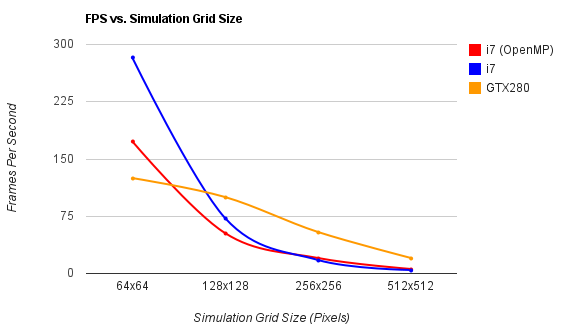
\includegraphics[scale=0.5]{chart}
\caption{FPS vs. Simulation Grid Size}
\end{figure}

The discrepancy between the results in Lee et al.'s paper and those previously reported by other authors can be attributed to a number of factors. One such factor is which CPU and GPU are being compared. Some studies have not made use of the best available CPU which results in inaccurate results. Another major factor is the degree to which software is optimized for each platform. Typically, when writing code for the GPU the architecture forces the programmer to phrase their problem in terms of optimal computation structure for the GPU. Conversely, because the CPU is able to run general purpose code, it is possible to create unoptimized software that will still execute. In a fair comparison, software must be properly optimized for both platforms.

\section{Performance Analysis}

\subsection{External Memory Bandwidth}

All computation requires that some amount of off die memory be brought to the processor for computation. The rate at which this can be accomplished is bound by the available bandwidth. Thus performance is generally bound by two factors. First, the application requires enough computation capability to fully process data from each memory access before the next fetch cycle. Second, performance hinges upon the working set fitting into on-die caches (or buffers). In their research, Lee et al. found that the SAXPY and LBM applications have large working sets and therefore are purely bandwidth bound. These applications, as well as any other bandwidth bound applications, primarily benefit from increased bandwidth. Results for these applications (5.3X and 5X respectively) are in line with the bandwidth difference of 4.7X between the i7 and GTX280. The SpMV application which Lee et al. examined has a large data set but very little computation. We note however that the GTX280 is only 1.9X faster faster for this application than the i7 which is 2.3X lower than the ratio of their bandwidths. This can be accounted for by the fact the SpMW application must keep vector and column matrix data in main memory as it cannot fit in the GPU on-chip shared buffer. However, on the CPU this data will end up in the caches resulting in better memory performance on the CPU. In the case of our fluid simulation it was necessary to copy back the density buffer information to the GPU in order to then draw it using OpenGL. In the case of a buffer of 512x512 32-bit floating point numbers this requires approximately 1MB of memory be copied from the GPU memory to CPU host memory for each frame update. While this is a seemingly insignificant amount of memory compared to the bandwidth available on the GPU, the transfer requires that the GPU drivers synchronize and lock the memory as it is transfered which adds significant latency. 

\subsection{Maximum Effective Compute Flops}

Computational performance is dependent upon single thread performance but also thread level parallelism in the case of multiple cores being available as well as data level parallelism for hardware with SIMD facilities. While nearly all applications (expect those that are bandwidth bound) can benefit from additional single thread performance not all applications can take advantage of multiple thread and SIMD operations so easily. Amongst the applications presented by Lee et al., the SGEMM, MC, convolution, FFT and Bilateral filtering were identified as being able to exploit all available FLOPS on GPU and CPU hardware when optimally implemented. In the case of SGEMM, Conv and FFT the performance delta is 2.8-4X which is in line with the single-precision FLOP ratio of the GTX280 and i7. However, the GPU still cannot achieve its theoretical max FLOPS as the applications depend on a shared buffer. Monte Carlo method requires double-precision and therefore has a performance ratio of 1.8X which is close to the 1.5X delta of double-precision FLOP for CPU and GPU. Due to the use of fast transcendental functions, Bilateral filtering is able to achieve 5X performance on the GPU vs. the CPU. Interestingly, the radix sorting operation is bound by the SIMD width of the processor as the typical implementation requires reordering data involving many scalar operations for buffer management. As scalar code is inefficient on the GPU the GPU is actually 1.25X slower. We used the NVidia Visual Compute Profiler to examine the bottlenecks in our GPU implementation and found that our GPU implementation was bound by the time required to write back computed results to memory and that we were not able to achieve peak FLOPS. However, in the case of reading from multiple memory locations in memory, we were able to use the texture sampling functions which automatically coalesce accesses preventing the slowdown we experienced on writes.

\subsection{Cache Utilization}

The presence of on-die cache can alleviate the performance penalty from bandwidth pressure to external memory. When the working set of an application fits within the caches nearly all applications are compute bound. Some applications such as radix sort cannot have their working set size modified. Radix sort performs better on the CPU than GPU as a result of larger on-die caches despite the GPU having greater FLOPS. In the case of search, when the tree is small, the entire working set can reside in CPU cache resulting in the CPU being faster than the GPU. On large trees, however, the GPU is faster because it has greater bandwidth to its DDR memory. The Lee et al. paper examines those kernels with working sets that scale with the number of threads. For example, ray casting becomes bandwidth bound as the dataset increases beyond what the small amount of on-die shared memory can cache. Similarly, our results show that when the fluid simulation grid size is small and fits nicely with the cache size, the CPU solution outperforms the GPU. As the grid size grows the GPU begin to have an advantage due to its greater external memory bandwidth. We note that since the GPU doesn't have a cache its performance scales roughly linearly whereas the CPU performance drops off precipitously once the working set exceeds what fits in the available cache. (Fig. 5)

\subsection{Gather/Scatter Operations}

For kernels that are not already bandwidth bound, additional performance can be achieved through data level parallelism. In order to use SIMD instructions, it is necessary to group together  or gather operands into a block of sequential memory. For example, on four wide single-precision SIMD the processor expects four 16-byte aligned blocks. If the required data does not happen to conveniently be in this arrangement then additional operations must be expended in performing the arrangement. This operation of collecting and arranging data is referred to as a "gather." After the SIMD operation is completed, a reverse "scatter" operation is then required to move the results to their respective locations. These additional gather/scatter operations can result in significant processing overhead.

\subsection{Reduction and Synchronization}

High performance throughput computing is achieved through thread and/or data level parallelism. This is relatively easy to implement when the data being processed is independent. That is, the results from one thread are not needed in another thread. If this is not the case then synchronization and reduction are required. These operations are difficult to implement on parallel processing hardware. In the case of histogram calculation the main limitation is performing the atomic updates of intermediate results. As a result, on the GPU the histogram is computed in parts before a final summation. However, this reduction approach does not scale well with an ever increasing number of processor units. The constraint solver application is actually 1.9X slower on the GTX280 as a result of not having the relatively efficient cache coherency hardware that is found on the Core i7. Because there is no cache coherency hardware on the GPU, it must launch multiple batches from the CPU, severely hindering performance. 

\subsection{Fixed Function Units}

Many applications make extensive use of transcendental operations such as computing exponents and power functions. In many cases, such as image processing, where quality is subjective, the precision of these operations is not critical. Because the CPU is used for general purpose computation, it cannot make assumptions about the accuracy the programmer requires and therefore uses full precision algebraic expressions for these operations. As the GPU is designed for graphics, it simply implements fixed function equivalents in hardware. Additionally, the GPU implements filtered multi-sampling in hardware, which accelerates data sampling in graphics applications where multi-sampling is typically used.

\section{Software Optimization Suggestions}

Historically, CPU performance has been improved by increasing the clock frequency. As it becomes more difficult for CPU designers to increase the clock speed, it is becoming increasingly important for programmers to take advantage of thread and data level parallelism to achieve maximum performance in their applications. It is observed that most applications can achieve  performance improvements nearly linear with the number of cores through the use of strategic multi-threading. The CPU suffers from relatively low memory bandwidth and as a result is dependent on its caches for performance. This requires the programmer to use blocking techniques to ensure that the working set data is formatted to fit nicely within the caches. Similarly, as the CPU lacks efficient gather/scatter support, it is necessary to re-order instructions to prevent random memory access in order to achieve better performance. 

The GPU is most penalized by global inter-thread synchronization as it can only be handled by kernel termination and re-issuing. GPUs can gain additional performance by making good use of the shared buffer to reduce overall bandwidth consumption. Furthermore, the shared buffer is multi-banked and can be used to implement efficient gather/scatter operations.

\section{Hardware Design Suggestions}

Based upon our performance results and analysis of current generation CPU and GPU hardware, we propose examination of the following areas in order to improve parallel processing performance on future generations of hardware.

\subsection{Increased FLOPS Through Core Count and SIMD Width}

Raising the effective FLOPS can be achieved through some combination of increasing the number of cores and/or increasing the SIMD width. The number of cores is limited by the size of the die. Increasing the SIMD width is often a better approach as it requires relatively less additional space on the CPU die. This logic is borne out in recent hardware trends with both Nvidia and Intel opting to increase SIMD on their forthcoming devices. However, SIMD can only improve efficiency when memory access is regular and the full width is utilized effectively. 

At the same time, raw FLOPS are only useful when they are matched with sufficient bandwidth to get the data to the computation hardware. Current GPUs attempt to achieve this bandwidth through the use of expensive GDDR memory which limits the amount that can economically be placed on the card. Additionally, adding ever greater sums of memory results in greater power consumption. Promising memory technologies such as 3D-stacking and cache compression may be able to help increase bandwidth in future.

\subsection{Optimize Cache Size}

For optimal performance, the size of on-die caches should match the working set size of typical applications. For nearly all current applications an on-die cache of 8MB is sufficient. However, as data sizes increase, further larger caches may be required.

\subsection{Explicit Gather/Scatter Hardware}

Application performance presented in the paper suggests that there are significant performance gains possible through efficient gather/scatter support. An ideal gather operation would simultaneously gather all elements into an SIMD register in the same time requires to load a single cache line. An implementation of the idealized gather may be impractical as it would require a large number of cache ports. The GTX280 uses multi banking to achieve a similar effect by using a shared local memory which allows 16 simultaneous reads to 16 banks in one cycle. However, the structure is explicitly managed by the programmer leading to additional implementation complexity. 

\subsection{Efficient Synchronization and Cache Coherence}

The Core i7 processor has atomic locking on instructions such as increment and compare and exchange. The GTX280 only supports atomic operations through device memory. In both CPUs and GPUs current solutions to the synchronization problem do scale well. In future, as core counts and SIMD width increase better solutions will be required. Typically two types of synchronization are required in throughput computing: reductions and barriers. In order to efficiently handle reductions atomic vector read-modify-write hardware operations would need to be implemented. Faster barriers would improve performance in cases where task size is small in comparison to the number of cores. For tasks that require only thousands of cycles, barrier operations may still require hundreds of cycles. Fast hardware barriers would help guarantee memory consistency between caches.

\subsection{Implement Fixed Function Units for Common Specialized Tasks}

Fixed function hardware, such as dedicated transcendental units, can help improve performance in cases where they are frequently used, such as in filtering applications. Purpose built texture sample/multi-sampling units are effective in increasing performance in applications such as image and video performance. It is expected that as transistor size decreases it will be possible for more specialized hardware to be on-die.

\section{Conclusion}

Through our independent comparison of GPU and CPU performance, we found that for sufficiently large data sets exhibiting computational parallelism it is possible to achieve superior performance using GPU hardware for general purpose computation. However, the aforementioned qualifications are significant caveats and imply that only certain tasks are suitable for the GPU. In the specific case of fluid simulation, our results suggest that the GPU is an appropriate architecture, producing superior performance. Our results corroborate the findings of the prior study conducted by Lee et al. Having examined current GPU and CPU architectures we predict that the distinction between the two architectures will continue to be reduced as both converge on a common hybrid parallel processing architecture. In the case of the CPU, we expect to see a continuation of the trend of increasing core counts and SIMD width. In order to provide data to these processors we anticipate the development of larger caches as well as multi-ported memory systems that provide a hardware solution to gather/scatter bottlenecks. In the case of the GPU we anticipate the development of more efficient methods to provide thread synchronization. Additionally, new programming language features will need to be developed in order to make it possible for mainstream programmers to take advantage of GPU hardware.

\begin{thebibliography}{1}
\bibitem{Lee:2010:DGV:1816038.1816021}Lee, Victor W. and Kim, Changkyu and Chhugani, Jatin and Deisher, Michael and Kim, Daehyun and Nguyen, Anthony D. and Satish, Nadathur and Smelyanskiy, Mikhail and Chennupaty, Srinivas and Hammarlund, Per and Singhal, Ronak and Dubey, Pradeep, "Debunking the 100X GPU vs. CPU myth: an evaluation of throughput computing on CPU and GPU", SIGARCH Comput. Archit. News, vol. 38, pp. 451-460, 2010.
\bibitem{Stam:2003}Stam, Jos, "Real-Time Fluid Dynamics for Games", Proceedings of the Game Developer Conference, 2003.
\bibitem{Asanovic:2006}K. Asanovic, R. Bodnik, B. C. Catanzaro, J. J. Gebis, P. Husbands, K. Keutzer, D. A. Patterson, W. L. Plishker, J. Shalf, S. W. Williams and K. A. Yelick, "The landscape of parallel computing research: A view from berkely", Technical Report UCB/EECS-183, 2006.
\bibitem{Bienia:2008}C. Bienia, S. Kumar, J. P. Singh and K. Li, "The PARSEC benchmark suite: characterization and architectural implications", PACT '08: Proceedings of the 17th international conference on Parallel architectures and compilation techniques, pp. 72-81, ACM, New York, NY, USA, 2008.
\bibitem{Chen:2008}Y. K. Chen, J. Chhugani, C. J. Hughes, D. Kim, S. Kumar, V. W. Lee, A. D. Nguyen and M. Smelyanskiy, "Convergence of recognition, mining and synthesis workloads and its implications", Proceedings of the IEEE, 96(5):790-807, 2008.
\bibitem{IMPACT}The IMPACT Research Group, UIUC, "The Parboil benchmark suite", http://impact.crhc.illinois.edu/parboil.php.
\bibitem{Sanders:2001}Sanders, Jason and Kandrot, Edward, "CUDA by Example: An Introduction to General-Purpose GPU Programming", Addison-Wesley, Pearson Education, 2010.
\end{thebibliography}

\end{document}